\documentclass[10pt,twocolumn,letterpaper]{article}

% Мои собственные вещи
\usepackage{booktabs}
% \usepackage{caption}
% \captionsetup[table]{skip=8pt}   % Влияет только на таблицы
\usepackage{stfloats}  % Добавьте это в преамбулу
\usepackage{float}

\usepackage[T2A]{fontenc}    % Enables Cyrillic fonts
\usepackage[utf8]{inputenc}   % Assumes your source file is in UTF-8 encoding
\usepackage[russian]{babel}   % Loads Russian language support

% \makeatletter
% \def\cvprsubsection{\@startsection {subsection}{2}{\z@}
%     {8pt plus 2pt minus 2pt}{6pt}{\bfseries\normalsize}}
% \makeatother

\usepackage{cvpr}
\usepackage{times}
\usepackage{epsfig}
\usepackage{graphicx}
\usepackage{amsmath}
\usepackage{amssymb}

% Включайте здесь другие пакеты, перед hyperref.

% Если вы закомментируете hyperref, а затем раскомментируете его, вам следует удалить
% egpaper.aux перед повторным запуском latex. (Или просто нажмите 'q' при первом запуске latex)
% run, let it finish, and you should be clear).
\usepackage[breaklinks=true,bookmarks=false]{hyperref}

\cvprfinalcopy % *** Uncomment this line for the final submission

\def\cvprPaperID{****} % *** Enter the CVPR Paper ID here
\def\httilde{\mbox{\tt\raisebox{-.5ex}{\symbol{126}}}}

\renewcommand{\tablename}{Таблица}
\renewcommand{\figurename}{Рисунок}   % or whatever you like instead of "Hình"
\renewcommand{\refname}{Список литературы}

\makeatletter
\def\abstract{%
  \centerline{\large\bf абстракт}% <-- your new label
  \vspace*{12pt}%
  \it%
}
\makeatother

% This makes the font slightly bigger than base (10) and bold in Subsection headings rather than using ptmb
\makeatletter
\def\cvprsubsection{%
  \@startsection{subsection}{2}{\z@}%
    {8pt plus 2pt minus 2pt}{6pt}%
    % {\normalfont\bfseries\selectfont}%
    {\normalfont\bfseries\fontsize{11}{13}\selectfont}%
}
\makeatother

% So this hardcodes the style for the numbers in the section/subsection headings so they're bold
\font\elvbf=ptmb scaled 1100
\font\elvbfs=ptmb scaled 1200
\makeatletter
% Section number: Large + bold
\renewcommand\thesection{%
  {\elvbfs\arabic{section}}%
}

% Subsection number: normalsize + bold + custom punctuation
\renewcommand\thesubsection{%
  {\elvbf
   \arabic{section}.\arabic{subsection}}%
}
\makeatother

% Pages are numbered in submission mode, and unnumbered in camera-ready
%\ifcvprfinal\pagestyle{empty}\fi
\setcounter{page}{1}
\begin{document}

%%%%%%%%% TITLE
\title{"ECDO" Руководство на основе данных Часть 1/2: Текущее понимание экзотермического разделения ядра и мантии и эффекта Джанибекова (ECDO) — теория «переворота Земли»}

\author{Чжунхо\\
Опубликовано в феврале 2025\\
Веб-сайт (скачать статьи здесь): \href{https://sovrynn.github.io}{sovrynn.github.io}\\
Репозиторий исследований ECDO: \href{https://github.com/sovrynn/ecdo}{github.com/sovrynn/ecdo}\\
{\tt\small junhobtc@proton.me}
% Для статьи, все авторы которой из одного института,
% опустите следующие строки до закрывающей ``}''.
% Дополнительные авторы и адреса можно добавить с помощью ``\and'',
% так же, как и второго автора.
% Для экономии места используйте либо адрес электронной почты, либо домашнюю страницу, но не оба
% \and
% xxx
% Institution2\\
% Первая строка адреса института2\\
% {\tt\small secondauthor@i2.org}
}

\maketitle
%\thispagestyle{empty}

%%%%%%%%% ABSTRACT
\begin{abstract}
В мае 2024 года псевдоанонимный онлайн-автор под именем “The Ethical Skeptic” \cite{0} поделился революционной теорией, названной Экзотермическое разделение ядра и мантии - эффект Джанибекова (ECDO) \cite{1}. Эта теория предполагает, что Земля ранее переживала внезапные катастрофические сдвиги своей оси вращения, что вызывало масштабные мировые наводнения, поскольку океаны переливались через континенты из-за инерции вращения. Кроме того, в ней представлен объясняющий геофизический процесс и данные, указывающие на то, что подобный переворот может случиться снова в ближайшее время. Хоть и подобные предсказания о катастрофических потопах и конце света не новы, теория ECDO выделяется своим научным, современным, междисциплинарным и опирающем на данных подходом.

Эта статья является первой частью краткого изложния из двух частей за шесть месяцев независимого расследования \cite{2,20} теории ECDO. Оно подчеркивает три ключевых момента:

\begin{flushleft}
\begin{enumerate}
    \item ECDO-подобный «переворот Земли» происходил несколько раз в недавней истории человечества, о чём свидетельствуют мифы о потопе и геологические признаки широкомасштабных затоплений континентов.
    \item Приблизительное направление и величина прошлых переворотов Земли могут быть определены.
    \item Последние данные по геомагнетизму и геофизике указывают на еще один переворот Земли может произойти в ближайшее время, и что изменение климата может быть вызвано изменениями, происходящими глубоко внутри Земли, а не деятельностью человека.
\end{enumerate}
\end{flushleft}

Кроме того, я рассматриваю физическую природу, лежащую в основе «переворота Земли», предложенного теорией ECDO.

В этой статье я сохраняю объективность, опираясь на твёрдые данные, избегаю убедительных, но спекулятивных частей теории и подчёркиваю, что это тема, которую человечеству крайне важно стоит дальше изучать.
\end{abstract}

%%%%%%%%% BODY TEXT
\section{Введение}

Истории о великом потопе не новы — на самом деле, их можно найти в каждой крупной культуре по всему миру, охватывая все рамы цивилизации. График (рисунок \ref{fig:1}), компиляция из 267 историй о потопе \cite{3}, показывает, что практически на всех обитаемых территориях Земли существуют рассказы о потопах.
```latex
% \begin{figure}[h]
% \begin{figure}[b]
\begin{figure}[h]
\begin{center}
% \fbox{\rule{0pt}{2in} \rule{0.9\linewidth}{0pt}}
   \includegraphics[width=1\linewidth]{b.png}
\end{center}
   \caption{Места возникновения легенд о потопах по всему миру \cite{3}.}
\label{fig:1}
\label{fig:onecol}
\end{figure}

Более пристальный взгляд на эти легенды о потопах показывает, что это были не обычные наводнения, а разрушительные катастрофы, сопровождающиеся наводнениями, которые полностью очистили континенты.

\subsection{Истории катастроф коренных американцев}

Истории коренных американцев содержат одни из самых ярких описаний великих катастроф Земли. Хопи, племя коренных американцев, проживающее на северо-востоке Аризоны, говорит, что, \textit{"...Сотуктан сделал призыв к Муравьиным Людям открыть их подземный мир для избранных людей. Когда они были в безопасности под землей, Сотуктан приказал близнецам, Пекангхоя и Палонгауоя, покинуть свои посты на северном и южном концах оси мира, где они находились, чтобы поддерживать правильное вращение Земли. \textbf{Близнецы едва покинули свои посты, как мир, оставшись без никого чтобы его которолировать, потерял равновесие, закрутился в сумасшедшем вихре, а затем перевернулся дважды.} Горы с великим всплеском погрузились в моря, моря и озера захлестнули землю; и когда земля закрутилась по холодному и безжизненному космосу, она замерзла в твердом льду"} \cite{4}.

Многие из этих историй точно описывают грандиозный масштаб наводнений, рассказывая, как океаны поднялись и затопили всё, кроме самых высоких горных вершин. Индейцы скокомиш, живущие в штате Вашингтон, рассказывают, как, \textit{"Великий Дух, рассердившись на нечестивость людей и животных, решил избавить землю от всех, кроме хороших животных, одного доброго человека и его семьи. По указанию Великого Духа человек запустил стрелу в облако, затем другую стрелу в ту стрелу, и так далее, пока не получилась веревка из стрел от облаков до земли. Хорошие животные и люди поднялись наверх. Плохие животные и змеи начали подниматься, но человек оборвал веревку. \textbf{Тогда Великий Дух вызвал множество дней дождя, и вода затопила землю до снеговой линии Тахомы (гора Рейнир).} Когда все плохие люди и животные утонули, Великий Дух прекратил дождь, вода медленно спала, и хорошие люди и животные спустились на землю"} \cite{3}. Для справки: гора Рейнир — это действующий вулкан в штате Вашингтон с высотой вершины 4392,5 м над уровнем моря.
```
История о потопе у индейцев маках из штата Вашингтон конкретно упоминает многослойный (многоэтапный) потоп с очень тёплыми водами, что указывает на то, что это был вовсе не обычный потоп: \textit{"Океан поднялся так высоко, что отрезал мыс. Затем он отступил, достигнув самого низкого уровня через четыре дня, оставив бухту Неа-Бей на высоте и сухой. Затем он снова поднялся, покрыв все, кроме вершин гор. \textbf{Восходящие воды были очень теплыми.} Люди с каонэ, загрузив свое имущество, поплыли далеко на север. Многие погибли, когда их каноэ застряли в деревьях. Спустя еще четыре дня море вернулось в прежнее состояние, и люди обнаружили себя далеко на севере, где и поныне живут их потомки"} \cite{3}.

\subsection{Китайские истории о катастрофах}

На другой стороне Тихого океана, современная китайская цивилизация, как считается, началась с великого потопа. Династия Ся, по оценкам, существовавшая около 2000 года до нашей эры, была основана Юем Великим, который остановил Великий потоп Гунь-Юя \cite{6}. Во время его правления, \textit{"... говорится, что произошло чудо — солнце в течение десяти дней не заходило, леса воспламенялись, и появилась масса мерзких тварей... Огромная волна, которая "достигла неба" обрушилась на землю Китая. \textbf{"Вода достигала высоких гор, и подножия холмов совсем не было видно"}... "Разрушительны в своем разливе были воды наводнения," — говорил император. — "В своем огромном объеме оно охватывает холмы и покрывает вершины, угрожая небесам своим потоком." Император приказал приложить все усилия, чтобы открыть выходы для воды, застрявшей в долинах между горами. В течение многих лет население трудилось, стараясь освободить равнины и долины от наводнения, копая каналы и сливая воду с полей. На протяжении значительного числа лет все усилия были напрасны. Министр, отвечавший за это срочное и грандиозное дело, Кхуань, был приговорен к смерти из-за своей неудачи... и его единственный сын Юй сумел осушить землю. Это достижение было так высоко оценено, что Юй стал императором Китая после Ван Шуня, первого преемника Яхоу"} \cite{5}.

Похоже, что затоплению подвергся не только Китай, но также возникла необходимость пересчитать основное направление света и движения Солнца и Луны, что подразумевает изменение вращения Земли во время потопа: \textit{\textbf{"Этот император отправил ученых в разные края Китая и даже в Индокитая, чтобы определить расположение севера, запада, востока и юга, наблюдая за направлением восхода и заката солнца, а также за движением звезд.} Он также поручил своим астрономам выяснить продолжительность сезонов и составить новый календарь... "И тогда Яоу [Яхоу] повелел Хэ и Хо, в благоговейном согласии с великим небом, высчитывать и изображать движения и явления солнца, луны, звезд и зодиакальных созвездий; и уважительно передавать времена года народу""} \cite{5}.

Записи о катаклизмах в китайской истории на самом деле восходят гораздо раньше династии Ся, достигая эпохи Трех властителей и Пяти императоров \cite{7}. Нюйва, одна из Трех властителей и центральная фигура Сотворения в китайской истории, остановила потоп во время катастрофы, когда Земля изменила вращение: \textit{"Произошла ссора между двумя из могущественных богов, и они решили разрешить ее боем. Когда бог воды Гунь Гун увидел, что проигрывает, он ударился головой о гору Бучжоу — столп, поддерживающий небо. \textbf{Столп обрушился и вызвал наклон неба к северо-западу, а земли — к юго-востоку.} Это вызвало великие бедствия, такие как нескончаемые пожары, гигантские наводнения и появление свирепых людоедских чудовищ. Нюйва отрезала ноги гигантской черепахи и использовала их, чтобы заменить рухнувший столп, облегчая ситуацию и заделав небесную брешь камнями семи разных цветов, но ей так и не удалось полностью выправить наклоненное небо"} \cite{8}.

\subsection{Европейские, майянские, ближневосточные и юго-восточноазиатские истории о катастрофах}

Поскольку описать все истории о катастрофах в данной статье невозможно, я приведу краткое упоминание некоторых других заметных культур с подобными рассказами. В греческой литературе встречаются три истории о потопе: Деуалиона, Огига и Дардана \cite{9,10}. В первой из них, \textit{"После девяти дней потопа мир был разрушен, и ковчег остановился на вершине горы Парнас"}, высота которой составляет 2457 метров \cite{11}. Майянская литература считает, что до нынешнего Солнца существовало четыре разных Солнца, и что эпоха четвертого Солнца, Кальчиутлике, закончилась потопом, уничтожившим мир, около 3100 года до нашей эры, и рождением нынешнего пятого солнца \cite{12}. На Ближнем Востоке библейская хронология содержит известную историю о потопе Ноя, а в вавилонской поэме «Эпос о Гильгамеше» рассказывается похожий сюжет \cite{13}. Юго-восточноазиатские культуры также богаты историями о потопах — например, народ от Данум из Индонезии говорит, что, \textit{"Великий потоп однажды утопил многих людей. Немногие спаслись, сбежав в лодках на единственную горную вершину, оставшуюся над водой. Они прожили там три месяца, пока потоп не спал"} \cite{3}. Остров Борнео, на котором они живут, имеет максимальную высоту 4095 метров.

\begin{figure*}[b]
\begin{center}
% \fbox{\rule{0pt}{2in} \rule{.9\linewidth}{0pt}}
\includegraphics[width=1\textwidth]{marine.jpg}
\end{center}
   \caption{Глобальная карта морских (океанических) ископаемых, морской воды и солончаков/соляных рудников \cite{15,16,86,87}.}
\label{fig:2}
\end{figure*}

\subsection{Статистический анализ историй о катастрофах}

Очевидно, что эти истории описывают потопы, которые часто сопровождались другими видами катастрофических геофизических сил. Анализ 117 историй о катастрофах (Таблица \ref{tab: 1}) показывает, что огненные бури, изменения рельефа и изменения вращения Земли часто записаны как происходившие вместе с великими потопами \cite{14}:

\begin{table}[ht]
\begin{center}
\renewcommand{\arraystretch}{1.2}  % Опционально, для увеличения расстояния между строками
\begin{tabular}{|l|c|c|}
\hline
\textbf{Тип катастрофы} & \textbf{Количество} & \textbf{Процент случаев} \\
\hline\hline
Потоп/наводнение            & 84 & 71.79 \\
Огненная буря/пожар         & 39 & 33.33 \\
Топографические изменения     & 29 & 24.79 \\
Звёздные расстройства        & 15 & 12.82 \\
Обрушившееся небо           & 15 & 12.82 \\
Продолжительная тьма        & 14 & 11.97 \\
Потерянные земли и озера   & 12 & 10.26 \\
Циклоновые ветры           & 10 & 8.55  \\
Осевые/вращательные изменения  & 9 & 7.69  \\
Кипящие реки/озера/океаны  & 8 & 6.84 \\
\hline
\end{tabular}
\end{center}
\caption{Случаи катастрофических последствий в рассказах}
\label{tab: 1}
\end{table}

Специфичность преданий о потопе, появившихся у множества независимых культур по всему миру, наряду с совпадающими рассказами о других катаклизмах, указывает на то, что эти предания о потопе могут быть прямыми свидетельствами реально произошедших катастроф.

\section{Физические доказательства океанического потопа}

Дополняя предания о потопе, существуют различные формы физических доказательств широкомасштабного затопления океанами, находящихся на поверхности континентов Земли. Наиболее очевидными из них являются соль (морская вода, солончаки и соляные рудники) и морские (океанические) окаменелости, которые покрывают большие площади континентальной суши Земли. На рисунке \ref{fig:2} показано распределение морской воды (синий), солончаков и рудников (коричневый), а также морских окаменелостей \cite{15,16,86,87}, иллюстрируя масштаб этих признаков океанического затопления.

Одними из самых интересных районов, содержащих морскую воду, являются Гималайское нагорье Тибета и горы Анд в Южной Америке, обе территории имеют среднюю высоту 4000 метров, первая из них изображена на рисунке \ref{fig:3}. Истории наводнения Тибета гласят, что, \textit{"\textbf{Тибет был почти полностью затоплен}, пока бог Гья не сжалился над выжившими, не отвёл воды через Бенгалию и не послал учителей, чтобы цивилизовать людей, которые до этого были едва ли лучше обезьян"} \cite{3}. Перуанские мифы описывают процесс образования гор, происходивший одновременно с наводнениями, покрывавшими вершины гор: \textit{"Пастух со своими шестью детьми собрал всю пищу и овец, каких смог, и поднялся на вершину очень высокой горы Анкасмарка. \textbf{Во время того, как вода потопа поднималась, гора поднималась выше, так что ее вершина никогда не оказывалась под водой, а потом гора опустилась вместе с водой.} Шестеро детей заселили провинцию после потопа"} \cite{3}.

\begin{figure}[t]
\begin{center}
% \fbox{\rule{0pt}{2in} \rule{0.9\linewidth}{0pt}}
   \includegraphics[width=1\linewidth]{tibet.jpg}
\end{center}
   \caption{Топографическая карта Гималаев, показывающая морскую воду (бирюзовый), высохшую соль (белый) и морские окаменелости (красный) \cite{15,16,86,87}.}
\label{fig:3}
\label{fig:onecol}
\end{figure}

Хотя школа униформитаристов о геологии объясняет такие аномалии, как соль и морские окаменелости, длительными процессами, происходящими на протяжении миллионов лет, человеческие истории о потопах заставляют нас усомниться в этом подходе. Если бы океан действительно затопил континенты, то морская вода и морские окаменелости, легко обнаруживаемые на больших пространствах возвышенной земли, были бы именно тем, что мы ожидали бы найти.

\begin{figure*}[t]
\begin{center}
\includegraphics[width=0.85\textwidth]{khafre.jpg}
\end{center}
   \caption{Схема, показывающая дифференцированное, узорчатое карстовое выветривание, вызванное длительным, временным повышением уровня моря \cite{27}.}
\label{fig:4}
\end{figure*}

\subsection{Дополнительные физические аномалии}

Существуют многочисленные другие формы аномалий, которые униформитарная наука не может объяснить. Идеально сохранившиеся мгновенно замороженные мамонты, погребённые в иле, с мясом, пригодным к употреблению спустя тысячи лет \cite{17,18,19}, огромные пласты горизонтально отложенных осадков в Северной Америке, покрывающие 2,4 миллиона км$^2$ \cite{21}, рельефы мега-текущей ряби \cite{22} и неустойчивые камни, произошедшие за сотни километров, лежащие на вершинах гор \cite{23,26}, — это лишь некоторые из явлений, которые современная униформитарная геология просто отмахивает, используя универсальные объяснения "долгих, растянутых процессов". Такие аномалии лучше всего объясняются катастрофическими геофизическими силами, и они рассматриваются во второй части данной статьи.

Кроме того, экскурсии и реверсии геомагнитных полюсов широко признаны повторяющимся явлениями на Земле, на основании палеомагнитических данных \cite{35,40,41}. Однако современная наука не может точно объяснить, почему и как происходят эти реверсии полюсов.

\section{ECDO и пирамиды Гизы}

Пирамиды Хафра и Хеопса в Гизе — одни из ключевых точек в тезисе ECDO "Ethical Skeptic" \cite{27}, так как они не только представляют собой доказательства длительного временного океанического затопления, но также указывают на возможное направление флипов ECDO Земли, предполагая, что наши предки могли измерять катастрофы Земли и обладали инженерными навыками, чтобы зафиксировать эти знания в массивных, высокоинженерных каменных сооружениях. Эти две пирамиды, предположительно построенные около 2500 г. до нашей эры как гробницы для фараонов Хеопса и Хафры, обе находятся на севере Египта примерно на (30 С, 31 В). Их основания превышают 200 метров в длину, а высота — около 140 метров. Пирамида Хеопса была построена из примерно 2,3 миллиона известняковых блоков, каждый из которых весит в среднем более двух тонн \cite{24, 25}.

Существует большая неопределённость относительно происхождения этих пирамид, которую рассматривает Ethical Skeptic в своём тезисе. Он указывает на многочисленные несоответствия в общепринятом повествовании о пирамидах, предполагая, в лучшем случае, значительную путаницу в отношении возраста и истории пирамид:

\begin{flushleft}
\begin{itemize}
    \item Углеродное датирование древних строительных растворов и инструментов грабителей гробниц поблизости указывает на то, что пирамиды, вероятно, были построены гораздо раньше, чем считается в традиционной версии.
    \item Так называемые "карьерные метки", найденные во внутренних помещениях пирамиды Хеопса, являются подозрительными в их расположении, материале, степени сохранности, использовании египетских иероглифов и времени/обстоятельств обнаружения, что указывает на возможность подделки. Они также отличаются от других подлинных древних охристых надписей, найденных в другой части пирамиды.
    \item Дифференциальная карстовая эрозия рядом со Сфинксом не согласуется с традиционной версией касаемого его строительства.
\end{itemize}
\end{flushleft}

\begin{figure*}[b]
\begin{center}
\includegraphics[width=0.85\textwidth]{shafts.jpg}
\end{center}
   \caption{Внутренние шахты и камеры пирамиды Хеопса, которую Ethical Skeptic предлагает рассматривать как трёхчастную геофизическую обсерваторию для мониторинга событий ECDO \cite{28}.}
\label{fig:5}
\end{figure*}

Одной из ключевых областей исследования в тезисе Ethical Skeptic является дифференцированное, узорчатое эрозия на внешней стороне пирамиды Хафра, показанное на рисунке \ref{fig:4}. Верхушка пирамиды сохраняет свою оригинальную мягкую облицовку из туфового известняка, которая когда-то покрывала всю пирамиду. Эта облицовка на вершине пирамиды лишь слегка выветрена, но находится непосредственно над узким, сильно закарстованным слоем, раскрывающий более твёрдый известняк Моккатам (Mohs 7), использованный для внутренних конструкционных блоков пирамиды. Ниже этого слоя - тело пирамиды состоит из сильно закарстованного известняка Тура (Mohs 4). Ключевой момент здесь — то, что более мягкий туфовый известняк, использовавшийся во внешней облицовке пирамиды и состоящий из CaCO$_3$, может растворяться в воде при определённых условиях. Ethical Skeptic цитируется на селективное сильное карстовое выветривание, остановившееся на твёрдом известняке Моккатам, волнообразная эрозия по углам вершины, а также на разницу между слабо выветренной вершиной и сильным карстовым выветриванием нижней части пирамиды, как на явные доказательства выдержанного подъёма уровня океана, который затем быстро ушёл \cite{27}.

\begin{figure*}[b]
\begin{center}
% \fbox{\rule{0pt}{2in} \rule{.9\linewidth}{0pt}}
\includegraphics[width=1\textwidth]{drawing.jpg}
\end{center}
   \caption{Диаграма предлагаемой ротации ECDO на 104 градуса к северу вдоль 31-го восточного меридиана, где крестиками показаны восточная и западная точки поворота, а красным маркером обозначена пирамида Хеопса.}
\label{fig:6}
\end{figure*}

Ethical Skeptic также уделяет большое внимание внутреннему устройству и состоянию пирамиды Хеопса (рисунок \ref{fig:5}) в своем исследовании \cite{28}. Пирамида Хеопса содержит несколько помещений (Царская, Царицына и Подземная камеры), различные коридоры и шахты, а также две пары так называемых "воздушных шахт", по одной паре идущих от Царской и Царицыной камер \cite{29,30}. В этой статье мы рассмотрим только самые критичные части исследования Ethical Skeptic — ориентацию и дизайн двух пар "воздушных шахт", поскольку они содержат важную информацию о направлении переворотов ECDO Земли.

Важное здесь — понять, что шахты были построены, чтобы они очень точно указывали в сторону определенных направлений. Во-первых, обе пары шахт в настоящее время направлены строго на север и юг. Кроме того, каждая из них была построена с внутренним углом в 104 градуса.

Однако самой яркой уликой является небесная карта, вырезанная внутри в одной из шахт царицы. Эта звёздная карта ориентирована на небесный северный полюс на период примерно с 9600 по 9200 г. до нашей эры, с учётом прецессии равноденствий \cite{28}. Это указывает на намеренную ориентацию шахт, а также на то, что во время строительства одна пара шахт из покоев царя и царицы была направлена на небесный северный полюс. Это порождает вопрос — куда указывают другие концы шахт и почему обе они были построены с углом в 104 градуса? Ethical Skeptic предполагает, что они были построены для выравнивания с небесным северным полюсом после 104-градусного ECDO-переворота.

\section{Доказательства 104-градусного вращения вдоль 31-го меридиана}

Таким образом, Ethical Skeptic предполагает, что Земля испытывает периодические 104-градусные перевороты вдоль 31-го меридиана, вдоль которого расположена пирамида Хеопса и её двойные шахты. На рисунке \ref{fig:6} показано предполагаемое вращение, а также восточный (Индонезия, 121 градусов восточной долготы) и западный (Южная Америка, 59 градусов западной долготы) "шарниры", два места, которые не меняли своего положения после переворота вдоль 31-го меридиана. После перехода Земли в это новое состояние ожидается, что она останется там недолго (от нескольких десятилетий до веков), прежде чем вернуться к нынешнему "нормальному" состоянию \cite{150}.

Одна особенно интересная история о катастрофе рассказывается Геродотом, самым известным историком в Древней Греции, который жил в V веке до нашей эры \cite{31}. В своей книге "История" Геродот рассказывает, как египетские жрецы поведали ему: \textit{"...от первого короля до этого жреца Гефеста, который царствовал последним, прошло триста сорок одно поколение людей... а триста поколений людей равны десяти тысячам лет, ибо сто лет составляет три поколения людей... Таким образом, за одиннадцать тысяч триста сорок лет, сказали они, не возникал ни один бог в человеческом образе; и ни до этого времени, ни после среди оставшихся королей, которые правили в Египте, они не сообщали, что что-либо подобное случалось. \textbf{За это время, говорили они, солнце четыре раза меняло своё обычное место восхода, и там, где оно теперь заходит, оно дважды восходило, а в том месте, откуда сейчас восходит, оно дважды заходило;} и при этом в Египте ничто не изменилось от своего обычного состояния: ни то, что исходит из земли, ни то, что приходит из реки, ни то, что касается болезней или смертей"} \cite{32}. Жрец Гефеста может быть датирован началом VII века до н.э., так как он был современником Синаххериба, царя Новоассирийской империи, как утверждает сам Геродот \cite{32,33,34}.

Эта история важна, потому что она сообщает, что когда Солнце меняло своё положение в Египте, оно \textit{именно меняло место восхода и захода}. Такое могло произойти только если Египет перевернулся на 180 градусов, оставаясь на похожей широте. Учитывая конструкцию пирамид и данные, приведённые в следующем подразделе, можно предположить, что Египет находится на меридиане, вдоль которого Земля поворачивается в своё новое положение (31-й восточный меридиан).

Египет — это \textit{единственное} место на Земле, где история однозначно говорит о смене мест восхода и захода Солнца. На самом деле, единственная другая история на Земле, описывающая конкретное направление вращения Земли — это история Нюйва из Китая, в которой говорится, что, \textit{"Столб рухнул и заставил небо наклониться к северо-западу и землю сместиться к юго-востоку"} \cite{8}. Это направление вращения также соответствует предложенному направлению вращения.

\subsection{Физические доказательства 104-градусного вращения вдоль 31-го меридиана}

Физические доказательства, подтверждающие это направление вращения, включают палеомагнитные, тектонические, пустынные, биоразнообразие, палеотечения и ледниково-валунные данные.

Изучение палеомагнитных данных, фиксирующих траектории геомагнитных полюсов при событиях Исландского бассейна и Лашампских экскурсий \cite{35}, показанных на рисунке \ref{fig:7}, демонстрирует вращение полюсов примерно вокруг восточного ECDO-шарнира (0 С, 121 В). Эти данные сохраняются в определённых типах магнитных минералов в горных породах, сформировавшихся во время перемещений полюсов, сохранив информацию о направлении и напряжённости магнитного поля Земли в то время.
\begin{figure}[t]
\begin{center}
% \fbox{\rule{0pt}{2in} \rule{0.9\linewidth}{0pt}}
   \includegraphics[width=0.95\linewidth]{laj.jpg}
\end{center}
   \caption{Траектории виртуальных геомагнитных полюсов для (a) экскурсии исландского бассейнового и (b) Лашампской экскурсии \cite{35}.}
\label{fig:7}
\label{fig:onecol}
\end{figure}

\begin{figure}[t]
\begin{center}
% \fbox{\rule{0pt}{2in} \rule{0.9\linewidth}{0pt}}
   \includegraphics[width=1\linewidth]{meinesz3.jpg}
\end{center}
   \caption{Изображение схем сдвиговых структур в земной коре \cite{36}.}
\label{fig:8}
\label{fig:onecol}
\end{figure}
\begin{figure*}[t]
\begin{center}
% \fbox{\rule{0pt}{2in} \rule{.9\linewidth}{0pt}}
\includegraphics[width=0.95\textwidth]{biodiversity.jpg}
\end{center}
   \caption{Изображение основных пустынь мира и чередующихся центров биоразнообразия \cite{28}.}
\label{fig:9}
\end{figure*}

Исследование сдвиговых (разломных) плоскостей в земной коре (см. рисунок \ref{fig:8}), где земная кора была разрушена или деформирована, также следует той же закономерности. Феликс Мейнесс, нидерландский геофизик, поясняет в своей статье \cite{36}, что наиболее вероятной причиной возникновения этой закономерности является смещение оси вращения Земли.

Расположение основных пустынь и центров биоразнообразия мира также соответствует этой закономерности. Пустыни находятся в местах, где ожидается интенсивное накопление осадков, тогда как точки биоразнообразия располагаются в районах, которые в меньшей степени подвергаются воздействию океанических смещений \cite{28}. Это расположение показано на рисунке \ref{fig:9}.

Такие совпадения с предсказанным путём вращения ECDO также присутствуют в палеотечениях осадков, сохранившихся в слоях песчаника западной части Соединенных Штатов \cite{21}, а также в ледниковых валунах-эратиках, которые представляют собой камни, предположительно перемещённые ледниками и отложенные на коренной породе иного типа, чем сам валун. В Великобритании эти валуны следуют ожидаемым путям перемещения, соответствующим вращению по модели ECDO \cite{67,68}.

\section{Вызывающая физика в перевороте ECDO}

\begin{figure*}
\begin{center}
% \fbox{\rule{0pt}{2in} \rule{1\linewidth}{0pt}}

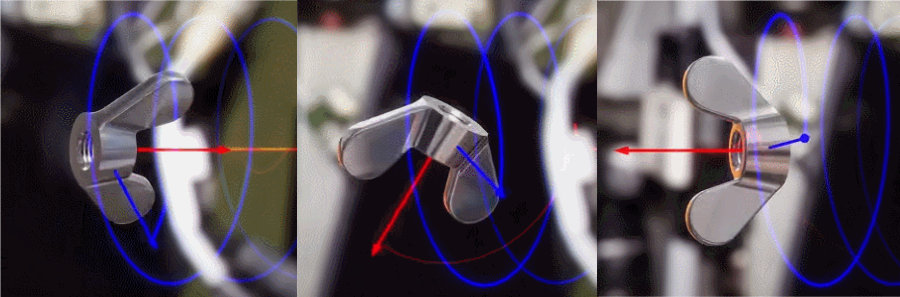
\includegraphics[width=0.9\textwidth]{dzhani.jpg}
\end{center}
   \caption{Изображение эффекта Джанибекова \cite{28}.}
\label{fig:10}
\end{figure*}

Принцип быстрого изменения оси вращения Земли заключается в физике вращающихся объектов. Каноническим примером этого является эффект Джанибекова, открытый русским космонавтом Владимиром Джанибековым \cite{37} и изображённый на рисунке \ref{fig:10}. Объект, который вращается не строго вокруг одной из трёх своих главных осей инерции, не будет сохранять фиксированную ось вращения. Если объект вращается по второй главной оси, он будет испытывать, как кажется, внезапные сдвиги в вращении. Хотя это не совсем то, что, по нашему мнению, происходит при быстрых переворотах Земли, важно то, что при отсутствии внешних сил только законы вращательного движения могут объяснить быстрое изменение оси вращения Земли.

Точнее говоря, Земля почти наверняка не испытывает простого и равномерного эффекта Джанибекова. Если бы это было так, мы могли бы зафиксировать постепенное смещение оси вращения Земли со временем. Скорее, мы считаем, что Земля испытывает периодические внезапные нарушения своей физической структуры, приводящие к расцеплению её "внешней вращающейся" (коры/мантии) и "внутренних вращающихся тел" (ядро). Без внешнего воздействия закон сохранения углового момента гласит, что Земля не может внезапно изменить свою ось вращения, поэтому расцепление внешних и внутренних вращающихся тел — одна из немногих вещей, за исключением внешнего удара по Земле, что может вызвать внезапный и резкий переворот.

Конкретный процесс, вызывающий внутреннее нарушение в недрах Земли, считается связанным с фазовым переходом в структуре железа, из которого состоит ядро Земли (см. рисунок \ref{fig:11}). Внутреннее ядро состоит из гексагонально-плотноупакованного железа (Fe) \cite{141}. По мере того как это hcp-Fe преобразуется в жидкое металлическое состояние, оно высвобождает кинетическую энергию и выталкивается во внешнее ядро. Этот фазовый переход уменьшает магнитную проницаемость ядра, ослабляя геомагнитное поле, и выделяет тепло, создавая структуры БОСНС (Большие области сдвига с низкой скоростью) (рисунок \ref{fig:12}) \cite{38} в мантии и нагревает поверхность Земли через абиссальные океаны. Оба этих процесса хорошо задокументированы в последние века и будут обсуждаться далее в этой статье.

\begin{figure*}[t]
\begin{center}
% \fbox{\rule{0pt}{2in} \rule{.9\linewidth}{0pt}}
\includegraphics[width=1\textwidth]{layers.jpg}
\end{center}
   \caption{Изображение внутренних процессов Земли, приводящих к перевороту ECDO \cite{129}.}
\label{fig:11}
\end{figure*}
\begin{figure}[t]
\begin{center}
% \fbox{\rule{0pt}{2in} \rule{0.9\linewidth}{0pt}}
   \includegraphics[width=1\linewidth]{llvp.jpg}
\end{center}
   \caption{Подробное изображение БОСНС под Южной Африкой \cite{28}.}
\label{fig:12}
\label{fig:onecol}
\end{figure}

Этот же процесс внутри Земли, происходящий в обратном порядке, также, как полагают, способствует возвращению к текущему состоянию вращения Земли относительно скоро после того, как происходит переворот.

\section{Доказательства надвигающегося переворота Земли}

Имеются веская причина верить, что мы находимся на пороге очередного переворота Земли. Катастрофа не происходила уже несколько тысячелетий, что примерно соответствует частоте этих событий, исходя из исторических свидетельств и данных. Самые убедительные данные, подтверждающие надвигающийся переворот, поступают из недавних геомагнитных данных, которые показывают, что геомагнитное поле Земли ослабевает примерно две тысячи лет. Это ослабление ускоряется и достигло тревожных темпов за последние несколько десятилетий.

На рисунке \ref{fig:14} показано геомагнитное поле Земли в 1590 и 2025 годах \cite{125,126}. Как видно на рисунке, поле значительно ослабло.
Другим показателем ослабления геомагнитного поля является положение геомагнитного северного полюса (Рисунок \ref{fig:13}). Геомагнитный север исторически располагался в канадской Арктике. Однако он медленно перемещался в течение последних нескольких столетий и значительно ускорился несколько десятилетий назад. Сейчас он быстро движется в сторону России со скоростью 55 километров в год. \cite{124}.

\begin{figure*}[t]
\begin{center}
% \fbox{\rule{0pt}{2in} \rule{.9\linewidth}{0pt}}
\includegraphics[width=0.9\textwidth]{saa.jpg}
\end{center}
   \caption{Изображение ослабления геомагнитного поля с 1590 по 2025 год. Расчитано с использованием моделей gufm1 и IGRF-14 \cite{125,126}.}
\label{fig:14}
\end{figure*}

\begin{figure}[t]
\begin{center}
% \fbox{\rule{0pt}{2in} \rule{1\linewidth}{0pt}}
   \includegraphics[width=1\linewidth]{npw.jpg}
\end{center}
   \caption{Положение геомагнитного северного полюса с 1590 по 2025 год, показано с шагом в 5 лет \cite{142}.}
\label{fig:13}
\label{fig:onecol}
\end{figure}

\begin{figure}[t]
\begin{center}
% \fbox{\rule{0pt}{2in} \rule{1\linewidth}{0pt}}
   \includegraphics[width=1\linewidth]{ocean-highlight.jpg}
\end{center}
   \caption{Темпы потепления глубинного океана ($>$2000 м глубины) с 1991 по 2010 год, обведены красным \cite{132}.}
\label{fig:15}
\label{fig:onecol}
\end{figure}

Считается, что магнитное поле Земли создается внутренним динамо — круговыми колоннами потоков магмы, движущихся во внешнем ядре Земли из-за её вращения \cite{123}. Ослабление геомагнитного поля является симптомом нарушений в глубинах Земли. Согласно теории ECDO, эти нарушения выбрасывают тепло и в конечном итоге приводят к развязке мантии и ядра, вызывая переворот Земли \cite{1}.

Существует значительное количество данных, подтверждающих наличие внутренних экзотермических процессов Земли. Потепление Земли зафиксировано в увеличении температур на континентальных и океанических поверхностях \cite{127,128}, росте уровня атмосферного CO2 синхронно с тепловыми струями Земли \cite{129,130}, а также сокращении площади мирового морского льда \cite{131}. Данные свидетельствуют о том, что рост концентрации CO2 и температур не являются причиной «антропогенного» изменения климата, а скорее следствием экзотермического ядра \cite{129}.

Наиболее существенно то, что исследования темпов потепления в глубоководных слоях океана (глубина $>$2000 метров) показывают: не только глубокие воды океанов разогреваются, но и самые высокие темпы потепления наблюдаются в абиссальном слое (4000–6000 м). Это потепление глубинных вод имеет центр ниже 4000 метров \cite{132,129}, что было бы невозможно, если бы океаны нагревались сверху атмосферой. Эти данные сильно поддерживают точку зрения, что недавние климатические и геомагнитные изменения вызваны процессами глубоко внутри Земли. На рисунке \ref{fig:15} показаны глобальные темпы потепления глубин океана с 1991 по 2010 год \cite{132}.

\section{Моделирование надвигающегося переворота Земли}

\begin{figure}[b]
\begin{center}
% \fbox{\rule{0pt}{2in} \rule{1\linewidth}{0pt}}
   \includegraphics[width=1\linewidth]{saa-crop.jpeg}
\end{center}
   \caption{Расчет критической точки на основе Южно-Атлантической аномалии указывает на дату 13 марта 2059 года \cite{125,126}.}
\label{fig:16}
\label{fig:onecol}
\end{figure}

Предсказывание время следующего переворота Земли — сложная задача. В настоящее время лучшей моделью для этого служит геомагнитное поле Земли — Южно-Атлантическая аномалия (ЮАА). Этот регион над Южной Атлантикой обладает самой слабой напряжённостью геомагнитного поля и определяется как область с напряжённостью ниже 32000 нанотесла \cite{135}, что было самым слабым значением поля в 1590 году. Площадь поверхности Южно-Атлантической аномалии увеличилась с 1\% поверхности Земли в 1590 году до 21\% в 2025 году \cite{136}.

Чтобы получить приблизительную оценку того, когда Земля может перевернуться, я поместил данные о площади поверхности ЮАА в уравнение использования степенной критической точки, которое моделирует сложную систему, приближающуюся к критическому переходу, при котором система претерпевает резкое и внезапное изменение. Мои расчёты дали прогнозируемую дату критической точки — 13 марта 2059 года (рисунок \ref{fig:16}). Эта предсказание будет становиться всё более точным по мере приближения к переходу \cite{136}.

Другие показатели, такие как блуждание оси вращения, погодные аномалии, сейсмические и вулканические данные, также могут помочь нам получить более точный прогноз того, когда может произойти следующий переворот Земли.

\section{Историческая хронология ECDO}

Хотя установить точную хронологию прошлых событий ECDO сложно, кажется, что в голоцене произошло по крайней мере 2 события ECDO. Обратите внимание на рассказ, переданный Геродотом от египетских жрецов: \textit{"от первого короля до этого жреца Гефеста, который правил последним, насчитывалось триста сорок одно поколение людей... За это время, говорили они, солнце четыре раза меняло своё обычное место восхода, и там, где оно теперь заходит, оно дважды восходило, а в том месте, откуда теперь восходит, оно дважды садилось"} \cite{32}. Платон, живший в V веке до нашей эры \cite{111}, утверждал, что после потопа, который затопил Атлантиду за один день и ночь 9 000 лет назад, \textit{"с тех пор было много потопов, а выжившие в горах не знали искусства письма и в течение многих поколений полностью были заняты только добыванием средств к жизни"} \cite{112}, что указывает на то, что после окончания Молодого Дриаса около 9700 года до нашей эры произошло более двух переворотов. Физические доказательства, рассмотренные в этой статье и в моих исследованиях \cite{2}, предоставляют достаточно доказательств рассказу Платона.

Самая последняя дата-кандидат на переворот ECDO приходится на период с 2300 по 1600 г. до нашей эры, к которому относятся многие описания катастрофических потопов (Гун-Ю \cite{113,114,115}, Огигес \cite{116,117}, Перу \cite{118,119}, Исход \cite{120}), разрушения и запустения цивилизаций (Мохенджо-Даро \cite{121}, Минойский Крит\cite{100,101}) и физические аномалии (события связи \cite{122}, событие 4,2 килогода \cite{90}). Нет достаточного совпадения доказательств более позднего периода, чем это, предполагающего крупное катастрофическое событие.

\section{Заключение}

"Операция Нанук" была разведывательной миссией Холодной войны, проведённой Соединёнными Штатами для картографирования Арктики и северного побережья Советского Союза после Второй мировой войны \cite{137}. В ходе расследования они обнаружили, что магнитный полюс находился на 125–200 миль севернее того места, где он должен был быть согласно результатам более ранних экспедиций. Соответственно, \textit{"Среди правительственных учёных возник вопрос: что произойдет, когда магнитный и географический полюса совпадут. Для ответа на этот вопрос под руководством доктора Пола А. Сайпла корпорация RAND была нанята для проведения лабораторных исследований с использованием моделей Земли, построенных из концентрических сфер — внутренняя сфера представляла электромагнитно-нагруженное расплавленное железное ядро Земли, ось которого определяла «магнитные» полюса; а внешняя сфера представляла земную кору, вращавшуюся вокруг «географической» полярной оси. В ходе многократных экспериментов было установлено, что по мере приближения «магнитного» полюса к «географическому» полюсу «магнитный» полюс в какой-то момент ускоряет свою скорость сближения, словно притягиваемый к «географическому» полюсу центростремительной силой, и совершает скачок для совпадения с ним; однако вместо совпадения полюсов «магнитный» полюс быстро «переваливает» вокруг «географического» полюса, затем словно по действием центробежной силы уходит к экватору, оказываясь в положении, когда две оси расходятся примерно на 89 градусов. После такого полярного «переворота» оси затем постепенно начинают повторно сближаться в течение долгого времени"} \cite{138,139}.

Впоследствии, \textit{"На одном из научных совещаний, которое майор Уайт посетил в Пентагоне в начале 1948 года, учёные обсуждали целесообразность информирования общественности о грядущем полярном перевороте. Ни один из учёных не согласился бы скрывать информацию от публики; но, с другой стороны, ни один из них не мог договориться, как это огласить. Знание об этом явлении, по мнению некоторых, само по себе может разрушить нравственные устои общества. Их опасения, как оказалось, были напрасны, когда в начале 1950-х годов информация о феномене переворота была опубликована и в газетной колонке, и в журнальной статье, но на удивление не вызвала никакой реакции со стороны, по всей видимости, ошеломлённой, провинциальной или недоверчивой публики"} \cite{138,139}.

Почему мы не обращаем на это внимания? Есть много оснований полагать, что Земля уже переворачивалась ранее. Эта статья, вместе с её второй частью, предоставляет ёмкое резюме большого сходства свидетельств из многих областей, указывающих на то, что это так: истории о потопах по всему миру, покров соли и морские окаменелости, покрывающие континенты, древние подземные убежища, останки животных и катастрофические геологические ландшафты. Как утверждается, человеку сотни тысяч лет, но новейшая история насчитывает лишь несколько тысяч лет. Не может ли быть так, что время от времени Земля переворачивается, континенты очищаются, и мы вынуждены возвращаться к исходной точке — каменному веку, и наши знания о древней истории сводятся к горстке катастрофических рассказов? Если это так, то предотвращение повторения этого может быть одной из важнейших задач человечества.

В заключение я оставлю вас с этим эпизодом, пересказанным в «Тимее» Платона, — беседой между Солоном, афинским государственным деятелем, и египетскими жрецами \cite{140}: \textit{"И в одном случае, когда [Солон] попытался склонить их к беседе о древней истории, он стал рассказывать им самые древние наши предания о Форонее, которого считали быть первым человеком, и о Ниобе; затем он рассказал легенду о Девкалионе и Пирре после Потопа, о том, как они спаслись, потом перечислил происхождение их потомков; и, пересчитывая число лет, занятых описанными событиями, попытался вычислить промежутки времени. Тут один из жрецов, чрезвычайно старый человек, сказал: «О Солон, Солон, вы, греки, всегда дети: нет у греков старика». И услышав это, он спросил: «Что ты подразумеваешь этим выражением?» И жрец ответил: «Вы молоды душой, все до одного. Потому что у вас нет ни единой древней и восходящей к традиции веры, также ни единой седой от древности науки. И вот причина тому: было и будет множество и всякого рода истреблений человечества, при которых крупнейшие совершаются огнём и водой, а меньшие — бесчисленными другими средствами. И действительно, рассказ, который передаётся у вас и у нас, как однажды Фаэтон, сын Гелиоса, запряг отцовскую колесницу и, не сумев её вести по тому пути, по которому ездит отец, сжёг всё, что было на земле, а сам погиб от удара молнии, — этот рассказ, как его рассказывают, имеет образ мифа, но истина его — в смещении движущихся вокруг земли небесных тел и в истреблении земных вещей яростным огнём, повторяющемся через долгие промежутки времени. В такие периоды все те, кто живёт в горах и на высоких и сухих местах, страдают от уничтожения больше чем те, кто живёт у рек или моря; а в нашем случае, Нил, наш Спаситель в других случаях, спасает и из этого бедствия поднимается высоко. А когда, с другой стороны, боги очищают землю потоками воды, то спасаются пастухи и скотоводы, живущие в горах, а жители ваших городов смываются потоками в море; у нас же вода никогда не льётся сверху на наши поля, напротив, она всегда, по природе своей, выходит из-под земли. Поэтому то, что у нас сохраняется, считается самым древним; правда заключается в том, что в местах, где нет излишнего холода или жара, всегда сохраняется какой-то человеческий род, то более, то менее многочисленный. И если где-нибудь происходит что-то славное, великое или заметное, будь то у вас, у нас или в каком-либо другом из известных нам мест, всё это отмечается с давних времён и хранится здесь, в наших храмах; у вас же и у других народов каждый раз всё начинается заново: письменность и другие искусства, необходимые цивилизованному государству. Однако, когда через обычный промежуток лет снова обрушивается, как болезнь, на ваш народ поток с неба, никто из вас не остаётся, кроме необразованных и невежественных, так что вы становитесь юными как прежде, не зная ничего о том, что происходило в древние времена — ни у нас, ни у себя. Действительно, те генеалогии, о которых ты только что рассказал, Солон, о людях своей страны, не менее лучше детских сказок: во-первых, ты помнишь лишь один потоп, несмотря на то что их было много; далее, ты не знаешь о том, что самый благородный и совершенный род среди людей родился на той самой земле, где сейчас живёшь ты, и от него произошёл и ты, и весь твой город, остаток из семени, уцелевший тогда; но это тебе неизвестно, потому что уцелевшие много поколений не могли оставить письменных свидетельств о себе. Ведь когда-то, Солон, до самого большого разрушения водой, афинское государство было самым воинственным и высокоорганизованным народом в отношении других. Говорят, оно обладало самыми выдающимися произведениями искусства и благороднейшей организацией, о каких мы слышали. Но об этом ты не знаешь ничего, потому что после великих потопов и катастроф на много поколений всё забывается»}.

Те же самые жрецы, конечно, рассказывали Солону и о древней цивилизации Атлантиды: \textit{"Всё, что находится здесь, внутри устья, о котором мы говорим, — это, по-видимому, гавань с узким входом; а то, что там дальше, — настоящий океан, и окружающая его земля правильнее всего называется континентом. На этом острове Атлантида существовал союз королей огромной и удивительной могущества, который владел всем островом, а также многими другими островами и частями материка; кроме того, на землях внутри пролива они властвовали в Ливии до Египта и в Европе до Тиррении. Вся эта армия однажды попыталась одним ударом поработить и вашу страну, и нашу, и всю территорию внутри проливов. Тогда-то, Солон, мужество твоего народа проявилось на весь мир: оно оказалось выше всех по доблести и военным искусствам — частично в роли лидера среди греков, а частично, стоя в одиночестве, когда все покинули его, выдержав страшнейшие испытания, оно победило захватчиков и воздвигло трофей; этим оно спасло от рабства ещё не порабощённых и всех остальных обитателей Геркулесовых столбов освободило. Но позднее произошли ужасающие землетрясения и наводнения, и одна страшная ночь и день постигло их, когда все тело ваших воинов было проглочено землей, а остров Атлантида так же оказался поглощён морем и исчез"}.

\section{Благодарности}

Благодарю Ethical Skeptic, оригинального автора работы по ECDO, за завершение его проницательной, новаторской диссертации и её публикацию для всего мира. Его трёхчастная работа \cite{1} остаётся основополагающей работой по теории экзотермического разделения ядра и мантии и эффект Джанибекова (ECDO), и содержит гораздо больше информации по теме, чем я успел изложить здесь.

Спасибо Анкиту, обработавшему данные по катастрофам в Таблице 1.

И, конечно, благодарности великанам, на чьих плечах мы стоим; тем, кто провёл все исследования и изыскания, которые сделали эту работу возможной, и кто трудился, чтобы принести свет человечеству.

\clearpage
\twocolumn

\section{Дополнительные изображения}


\begin{figure}[H]
\begin{center}
% \fbox{\rule{0pt}{2in} \rule{1\linewidth}{0pt}}
   \includegraphics[width=1\linewidth]{wave.jpg}
\end{center}
   \caption{Пристальный вид на подрез и параболическую волновую эрозию на пирамиде Хафры \cite{27}.}
\label{fig:19}
\label{fig:onecol}
\end{figure}

\begin{figure}[H]
\begin{center}
```latex
% \fbox{\rule{0pt}{2in} \rule{1\linewidth}{0pt}}
   \includegraphics[width=1\linewidth]{star-stone.jpg}
\end{center}
   \caption{Карта звёзд, вырезанная на камне в одном из шахт пирамиды Хеопса \cite{28}.}
\label{fig:20}
\label{fig:onecol}
\end{figure}

\begin{figure*}[t]
\begin{center}
% \fbox{\rule{0pt}{2in} \rule{.9\linewidth}{0pt}}
\includegraphics[width=1\textwidth]{deepsea.jpg}
\end{center}
   \caption{Визуализация аномалии нагрева в глубоких и абиссальных слоях океана по сравнению с обычной кривой атмосферного нагрева океана. Общая аномалия нагрева взята из NOAA \cite{147}, распределения нагрева в глубоких и абиссальных слоях из исследования Дебрюера \cite{132}, обработка данных и визуализация выполнены Ethical Skeptic \cite{129}.}
\label{fig:21}
\end{figure*}

\begin{figure*}[t]
\begin{center}
% \fbox{\rule{0pt}{2in} \rule{.9\linewidth}{0pt}}
```
\includegraphics[width=1\textwidth]{sealevel.jpeg}
\end{center}
   \caption{Уровень моря показывает увеличение дисперсии на 20\% за 75 лет на 63 станциях, что указывает на увеличение скорости течений. Всплески дисперсии уровня моря совпадают с пульсациями тепла в океане, что может свидетельствовать о нагреве из глубин под океанами Земли \cite{2,129}.}
\label{fig:22}
\end{figure*}

\begin{figure*}[t]
\begin{center}
% \fbox{\rule{0pt}{2in} \rule{.9\linewidth}{0pt}}
\includegraphics[width=1\textwidth]{co2.jpg}
\end{center}
   \caption{Концентрация CO2 в атмосфере (ppm) стабильно росла за последние 45 лет, вероятно, из-за повышения температуры океана. Источник: NOAA \cite{148,129}.}
\label{fig:23}
\end{figure*}

\begin{figure*}[t]
\begin{center}
% \fbox{\rule{0pt}{2in} \rule{.9\linewidth}{0pt}}
\includegraphics[width=1\textwidth]{ice.jpg}
\end{center}
   \caption{Глобальная площадь морского льда сокращается за последние 45 лет из-за потепления Земли. Источник: ADS \cite{149}.}
\label{fig:24}
\end{figure*}

\clearpage
\twocolumn

{\small
\bibliographystyle{ieee}
\bibliography{egbib}
}

\end{document}
